\documentclass[12pt]{article}
\usepackage[paperheight=210mm,paperwidth=148mm,top=2cm,bottom=2cm,left=1cm,right=1cm]{geometry}  % A5 paper
\usepackage{background}
\backgroundsetup{
scale=1,
opacity=0.1,
angle=0,
color=black,
contents={%

\includegraphics[width=\paperwidth]{background}
}
}
%%%%%%%%%%%%%%%%%%%%%%%%%%%%%%%%%%%%%%%%
\usepackage[utf8]{inputenc}
\usepackage{titlesec}
%\usepackage[all]{hypcap}
\usepackage{multirow}
%\usepackage{tikz}
\usepackage{ctable}
%%%%%%%%%%%%%%%%%%%%%%%%%%%%%%%%%%%%%%%%
\renewcommand{\familydefault}{\sfdefault}
% \titleformat{\chapter}[display]
% {\bfseries\LARGE\sffamily}{\chaptertitlename}{10pt}{\LARGE}
% \titlespacing*{\chapter}{0pt}{10pt}{10pt}
% \numberwithin{table}{chapter}


\begin{document}
% Cover
\newgeometry{left=0cm, bottom=0cm, top=0cm, right=0cm}
\thispagestyle{empty}
\noindent  % To remove the unwanted white space.
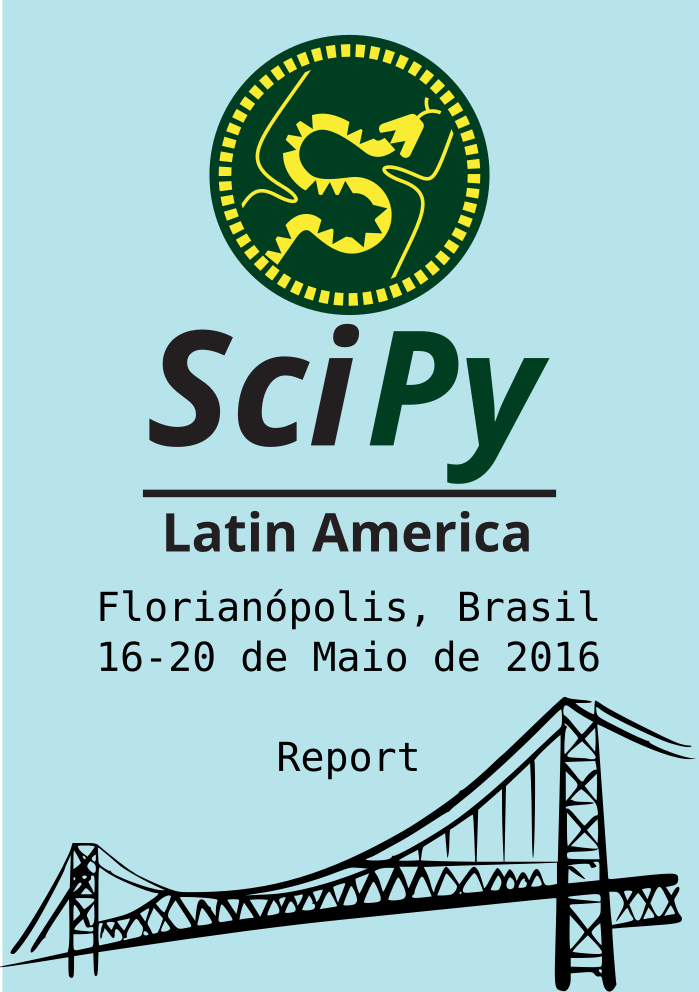
\includegraphics{capa}
\NoBgThispage

\clearpage

\restoregeometry

\newpage

\section*{Map of venue}


\newpage

Hi,

We welcome you to the 4th annual Latin American Conference on Scientific Computing with Python.
This year we will hosting one Software Carpentry workshop for beginners,
12 tutorials, 16 talks, 80 minutes for lightning talks
and some social events that includes an scavenger hunt.

The conference will start with an 40 minutes session for lightning talks
so that attendees could show their pet projects and have three days to talk with
those that will be interested on it.
On the course of the three days you can participate on the scavenger hunt
and try to win it's prize.

We hope that you enjoy your time in Florianópolis.
The Island of Santa Catarina has 42 beaches
and in the case you don't like beaches there is one lagoon.
Try to visit the Public Market
and the Fortress of São José da Ponta Grossa.

\textemdash\ Organizing Committee

\vfill

\hrule

\begin{center}
       \begin{tabular}{p{4cm} p{7cm}}
     Wi-Fi & Website: http://conf.scipyla.org/ \\
     SSID: eduroam & Twitter: http://twitter.com/scipyla/ \\
     Login: scipy & Hashtag: \textbf{\#SciPyLA2016} \\
     Password: SciPyla2016 & \\
   \end{tabular}
\end{center}



\newpage

\section*{Platinum Sponsors}
\begin{minipage}{0.4\textwidth}
COMPANY NAME

FOO

\end{minipage}
\hfill
\begin{minipage}{0.4\textwidth}
COMPANY NAME

FOO

\end{minipage}

\newpage

\section*{Gold Sponsors}
\begin{minipage}{0.4\textwidth}
COMPANY NAME

FOO

\end{minipage}
\hfill
\begin{minipage}{0.4\textwidth}
COMPANY NAME

FOO

\end{minipage}

% Space
\vspace*{1cm}

\begin{minipage}{0.4\textwidth}
COMPANY NAME

FOO

\end{minipage}
\hfill
\begin{minipage}{0.4\textwidth}
COMPANY NAME

FOO

\end{minipage}

\newpage

\section*{Tutorials - Overview}

\subsubsection*{16/05/2016}

\begin{center}
   {\footnotesize{%
     \begin{tabular}{@{}l p{5cm} p{5cm}@{}}
     \toprule
      & 9h-12h & 14h-17h\\\midrule
     Room 1 & \textbf{Python for geoscientist} (Filipe Fernandes) & \textbf{Utilización de Vispy para visualización rápida en 3D} (David Ochoa)\\
     Room 2 & \textbf{Introduction to MPI on python using mpi4py} (Jeudy Blanco) & \textbf{Introduction to High-Performance Scientific Computing with PyOpenCL} (Celia Cintas)\\
     Auditorium & \textbf{I see 42 everywhere} (Fernando Masanori) & \textbf{The stupid content tracker} (Tomas Aliaga)\\\bottomrule
   \end{tabular}
 }}
\end{center}

\subsubsection*{17/05/2016}

\begin{center}
   {\footnotesize{%
     \begin{tabular}{@{}l p{5cm} p{5cm}@{}}
     \toprule
      & 9h-12h & 14h-17h\\\midrule
     Room 1 & \textbf{Fit and predict your data: Introduction to Scikit-learn} (Celia Cintas) & \textbf{scikit-image: Realce e Detecção de bordas$^\star$} (Darleison Rodrigues)\\
     Room 2 & \textbf{Scientific Python applied to Petroleum Engineering - an Introduction$^\star$} (Igor T. Ghisi) & \textbf{Time Series Analysis Using Python$^\star$} (Bargava Subramanian)\\
     Auditorium & \textbf{Introduction to Data Analysis using Python Data Stack$^\star$} (Bargava Subramanian) & \textbf{Usando R com o Python - rpy2$^\star$} (Arnaldo Russo)\\\bottomrule
   \end{tabular}
 }}
\end{center}
{\footnotesize{$^\star$ Waiting for confirmation.}}

\subsubsection*{Locations}
{\footnotesize{%
\begin{description}
   \item[Room 1] Sala de Projeção Harry Laus (40)
   \item[Room 2] Sala de Projeção Henrique da Silva Fontes (24)
   \item[Auditorium] Auditório Elke Hering (80)
\end{description}
}}

\subsection*{Tutorials - Details}
\begin{description}
   \item[16/05/2016] \ 
   \begin{itemize}
      \item \textbf{Python for geoscientist}, \emph{Filipe Fernandes (ocefpaf@gmail.com)}. Intermediate. Sala de projeção Harry Laus, 9h-12h.
      \item \textbf{Utilización de Vispy para visualización rápida en 3D}, \emph{David Ochoa (ochoadavid@gmail.com)}. Intermediate. Sala de Projeção Harry Laus, 14h-17h.
      \item \textbf{Introduction to MPI on python using mpi4py}, \emph{Jeudy Blanco (jeudyx@gmail.com)}. Introductory. Sala de Projeção Henrique da Silva Fontes, 9h-12h.
      \item \textbf{Introduction to High-Performance Scientific Computing with PyOpenCL}, \emph{Celia Cintas (cintas.celia@gmail.com)}. Introductory. Sala de Projeção Henrique da Silva Fontes, 14h-17h.
      \item \textbf{I see 42 everywhere}, \emph{Fernando Masanori (fmasanori@gmail.com)}. Introductory. Auditório Elke Hering, 9h-12h.
      \item \textbf{The stupid content tracker}, \emph{Tomas Aliaga (tomas.aliaga@gmail.com)}. Introductory. Auditório Elke Hering, 14h-17h.
   \end{itemize}
   \item[17/05/2016] \ 
   \begin{itemize}
      \item \textbf{Fit and predict your data: Introduction to Scikit-learn}, \emph{Celia Cintas (cintas.celia@gmail.com)}. Introductory. Sala de Projeção Harry Laus, 9h-12h.
      \item \textbf{scikit-image: Realce e Detecção de bordas}, \emph{Darleison Rodrigues (darleison.f@gmail.com)}. Intermediate. Sala de Projeção Harry Laus, 14h-17h. \underline{(Waiting for confirmation)}
      \item \textbf{Scientific Python applied to Petroleum Engineering - an Introduction}, \emph{Igor T. Ghisi (igortg.subs@gmail.com)}. Introductory. Sala de Projeção Henrique da Silva Fontes, 9h-12h. \underline{(Waiting for confirmation)} 
      \item \textbf{Time Series Analysis Using Python}, \emph{Bargava Subramanian (bargava@gmail.com)}. Introductory. Sala de Projeção Henrique da Silva Fontes, 14h-17h. \underline{(Waiting for confirmation)}
      \item \textbf{Introduction to Data Analysis using Python Data Stack}, \emph{Bargava Subramanian (bargava@gmail.com)}. Introductory. Auditório Elke Hering, 9h-12h. \underline{(Waiting for confirmation)}
    \item \textbf{Usando R com o Python - rpy2}, \emph{Arnaldo Russo (arnaldorusso@gmail.com)}. Intermediate. Auditório Elke Hering, 14h-17h. \underline{(Waiting for confirmation)}
   \end{itemize}
\end{description}

\newpage

\subsection*{Tutorials - Abstracts}

%%%%%%%%%%%%%%%%%%%%%%%%%%%%%%%%%%%%%%%%%%%%%%%%%%%%%%%
\begin{description}
   \item[Title] \underline{Python for geoscientist}
   \item[Author] Filipe Fernandes \emph{(ocefpaf@gmail.com)}
   \item[Description] A tour, with some in depth examples, to the Geosciences Python software stack. The goal is to expose professionals and students to the state of the art Python libraries used for mapping, data exploration, data analyses, and visualization. This tutorial is aimed at intermediate Python users. 
   \item[Abstract] This tutorial won't focus in one tool, nor it is aimed to teach any tool from the ground up. The goal is to expose the attendees to a set of useful tools via applied examples. The ideal audience are intermediate users who can, after the tutorial, dig deeper and learn a new tool using the examples as a starting point. The tools we plan to cover are:
    NumPy: Basic file reading and array manipulation
    Pandas (GeoPandas, CTD, xarray): How to take advantage of the index for time-series analysis and the labeled columns to store important metadata.
    Seaborn: Basic stats plotting
    Statsmodels: Basic model fitting
    Dask: How to deal with arrays that don't fit in your laptop RAM.
    Rasterio, fiona, and gdal: GIS cheat-sheet
    Cartopy, folium: Mapping
    Iris: The Climate and forecast convention object in Python.
    Some oceanographic libraries tour: odvc, pyoos, pyugrid, pysgrid, ciso, utide, etc.
    Basic optimizations techniques: (a) ditch the for loop in NumPy. (b) Bring the for loop back with Cython and Numba.
    Using Python as a glue language: calling Fortran, R, MatlabTM, and octave from the Jupyter Notebook.
    \item[Speaker Bio] I grew up (mostly) in Southeast Brazil, but headed South to Universidade Federal do Rio Grande, where I received a Bachelor of Sciences in Oceanography. After college I attend the Universidade de São Paulo. I received a Masters of Science in Physical Oceanography in August 2005. I am currently a Ph.D. candidate in Marine Sciences at School of Marine Science and Technology.

I am got involved with open source the same way most of non-developers do: as a distraction from the Ph.D. and now it became my full-time job.

All the projects and organizations I am involved are on GitHub, so it is better ti just direct people to https://github.com/ocefpaf instead of writing a long bio ;-)
    \item[Info] Intermediate. 16/05/2016, Sala de Projeção Harry Laus, 9h-12h.
\end{description} 
%%%%%%%%%%%%%%%%%%%%%%%%%%%%%%%%%%%%%%%%%%%%%%%%%%%%%%%
\begin{description}
   \item[Title] \underline{Utilización de Vispy para visualización rápida en 3D}
   \item[Author] David Ochoa \emph{(ochoadavid@gmail.com)}
   \item[Description] VisPy es una librería OpenGL para Python (2, 3) que puede ser utilizada por programadores que conozcan de OpenGL o por científicos que necesiten una plataforma de visualización de alto nivel y alto desempeño. En este tutorial se desarrollará un ejercicio de visualización de múltiples con diferentes características (posición, velocidad, tamaño, color) en un espacio 3D bajo el paradigma de POO. 
   \item[Abstract] \begin{itemize} 
      \item La libería VisPy. VisPy inició cuando cuatro diferentes desarrolladores decidieron juntarse para hacer una sola librería de visualización: Luke Campagnola (PyQtGraph), Almar Klein (Visvis), Cyrille Rossant (Galry) y Nicolas Rougier (Glumpy). Ellos nos ofrecen una librería OpenGL de alto desempeño para Python (2, 3) que puede ser utilizada por programadores que conozcan de OpenGL o por científicos que necesiten una plataforma de visualización de alto nivel y alto desempeño. A pesar de estar todavía en desarrollo continuo, esta librería es estable y tiene un buen desempeño. La librería es altamente versátil y se apoya en los objetos de Numpy, siendo muy simple modificar los datos mostrados en la ventana gráfica con instrucciones del tipo:
      
\verb+visual.set_data(pos = new_position)+

Donde \verb+new_position+ es un arreglo numerico Numpy.

\item Tutorial: visualización de objetos esféricos en un espacio definido.

En este tutorial se desarrollarán dos partes:

    En la primera se presentarán algunas de las caracteristicas básicas de la librería y con estas se hará un sistema simple de presentación de objetos wireframe en un ambiente 3D. En este sistema se simulará el comportamiento múltiples de pelotas en volumen rectangular. Cada pelota es, en el código propuesto, un objeto y cada una de ellas tiene un comportamiento programado independientemente. Cada una de ellas controla, también, su propia contraparte en la visualización, que al igual que su posición y velocidad, es actualizada a cada timestep.

    Utilizando la misma plataforma de la primera en la segunda parte se desarrollarán objetos tipo burbuja. Estos son formados aleatoriamente en el fondo de un tanque y tienen un comportamiento diferente de las anteriores cambiando propiedades diferentes de tamaño y de color.

El tutorial no esta pensado en una visualización con el desempeño más rápido, sino para mostrar la utilización de la librería VisPy en una simulación programada en el paradigma POO, integrando naturalmente los objetos, sus características intrínsecas y su visualización.
\end{itemize}
    \item[Speaker Bio] Ingeniero mecánico y desarrollador de software. Actualmente trabajando en el proyecto de Doctorado con foco principal en algoritmos para la generación y evaluación de trayectorias de fresado para maquinas CNC (CAM). Apasionado en crear las herramientas computacionales correctas para resolver problemas complejos.

Mechanical engineer and software developer. Currently working in my Doctorate research project creating and evaluating toolpath generation algorithms for CNC milling (CAM). Passionate about creating the right tools for solving complex problems by coding.
    \item[Info] Intermediate. 16/05/2016, Sala de Projeção Harry Laus, 14h-17h.
\end{description} 
%%%%%%%%%%%%%%%%%%%%%%%%%%%%%%%%%%%%%%%%%%%%%%%%%%%%%%%
\begin{description}
   \item[Title] \underline{Introduction to MPI on python using mpi4py}
   \item[Author] Jeudy Blanco \emph{(jeudyx@gmail.com)}
   \item[Description] The goal of the tutorial is to introduce the participants to basic concepts of parallel programming using the MPI specification and the mpi4py library, going through several basic examples that cover the main features of the library. At the end of the tutorial, a practical exercise will be assigned to the participants.  
   \item[Abstract] MPI is widely used in the scientific community and is supported on several programming languages, python being one of them. The selected library is mpi4py which implements most of the MPI specification.

The tutorial will start with a brief description of parallel programming topics, including the different parallelism models such as data parallelism, tasks parallelism, introduction to beowolf clusters and the different paradigms in parallel programming and their approaches (OpenMP and MPI).

Then an historic overview of MPI, the main concepts (Communicators, Ranks) and the main library functions: \verb+MPI_Init+, \verb+MPI_Comm_size+, \verb+MPI_Comm_rank+, \verb+MPI_Send+, \verb+MPI_Recv+, \verb+MPI_Finalize+. Hand on examples covering all these functions will be presented to the participants, going from a simple Hello World to point to point communication and collective communication that covers Broadcast, Reduce, Scatter and Gather operations.

At the end of the tutorial, an exercise will be given to be solved in the class. A serial code for calculating Pi will be provided, and it will be the students task to parallelize it using mpi4py. The students will also have the opportunity to run benchmarks and compare the performance enhancement after parallelizing the code.
    \item[Speaker Bio] Professor and researcher at Centro de Investigaciones Espaciales, Universidad de Costa Rica. 8 years of experience as python developer and 4 years of experience working with MPI in different programming languages (Fortran, python). Professor of Scientific Computing with python at UCR where MPI with mpi4py is one of the course subjects. Administrator of the Chirripo cluster at UCR.
    \item[Info] Introductory. 16/05/2016, Sala de Projeção Henrique da Silva Fontes, 9h-12h.
\end{description} 
%%%%%%%%%%%%%%%%%%%%%%%%%%%%%%%%%%%%%%%%%%%%%%%%%%%%%%%
\begin{description}
   \item[Title] \underline{Introduction to High-Performance Scientific Computing with PyOpenCL}
   \item[Author] Celia Cintas \emph{(cintas.celia@gmail.com)}
   \item[Description] This tutorial will show how to build efficient hardware independent solutions (CPUs, DSP, FPGAs and GPUs) using PyOpenCL. The tutorial will give a brief introduction to the programming basics such as architecture, memory types, execution models. After the basic concepts, we will dive into PyOpenCL and how to use it to resolve parallel problems, from basic matrix operations to image processing. 
   \item[Abstract] OpenCL is an open, royalty-free standard for general purpose parallel programming across CPUs, GPUs. OpenCL let us develop fast and efficient code for a number of applications with different workload behaviors: control intensive (searching and sorting), data intensive ( image processing, simulation and modeling, and data mining), compute intensive (iterative methods, numerical methods and financial modeling).

OpenCL abstracts the code from specific hardware perks, allowing our programs to run over a wide range of hardware configurations. PyOpenCL is a Python programming environment, that reduce the amount of C code to only writing kernels, leaving the rest of our code (the host part) in Python, without renounce efficiency either speed and keeping hardware independence.

An overview of the tutorial structure:

\begin{itemize}
   \item What is GPGPU Programming?
   \item What is OpenCL? Components.
   \begin{itemize}
      \item Abstract Architecture of OpenCL
      \item Memory Types of OpenCL
      \item Execution Model of OpenCL
   \end{itemize}
   \item Introduction to PyOpenCL (hands-on)
   \begin{itemize}
      \item Getting information about our platform and hardware capabilities.
      \item Contexts
      \item Queue
      \item Kernel Code \& Programs
      \item Buffers (I/O)
      \item Practical examples:
      \begin{itemize}
         \item Basic matrix operations.
         \item Image processing.
         \item Fractal and multifractals computations.
      \end{itemize}
   \end{itemize}
\end{itemize}

Prior to the talk a github repo will be made available so attendees will be able to follow the talk. In the hands-on part the audience can run all the code shown in the talk and we will leave time to solve simple problems included in the tutorial.
    \item[Speaker Bio] PhD student in Computer Science working at CENPAT-CONICET on "Diversity, Systemic and Evolution" group. Focused on 2 and 3D landmarking, reconstruction and visualization. Free software advocate. Assistant Professor at UNPSJB in Fundamentals of Computer Science and Business Intelligence.
    \item[Info] Introductory. 16/05/2016, Sala de Projeção Henrique da Silva Fontes, 14h-17h.
\end{description} 
%%%%%%%%%%%%%%%%%%%%%%%%%%%%%%%%%%%%%%%%%%%%%%%%%%%%%%%
\begin{description}
   \item[Title] \underline{I see 42 everywhere}
   \item[Author] Fernando Masanori \emph{(fmasanori@gmail.com)}
   \item[Description] Hacking basic modules and classes to obtain the "Answer to the Ultimate Question of Life, the Universe, and Everything". The funny way to learn the importance of Free Software and inheritance and overloading in OOP or advanced topics like metaprogramming in Python. 
   \item[Abstract] Interactive tutorial for people, with the basics of programming, in some other language, and who know nothing of Python. Let's hack basic modules and classes to obtain the "Answer to the Ultimate Question of Life, the Universe and Everything." This tutorial assumes that you have a few basics (data input, data output, boolean operators, flow control, functions, repetitions). We will cover in Python 3: 1. The interactive Python mode 2. Variations in the guess the number game 3. Hacking basic modules and classes 4. Scraping Public Data in order to calculate World Cup costs 5. Chuck Norris nerd jokes and World Cup games in six lines of code. 6. Facebook Hackaton Selective Test in one line of code. Important note: I'm not a Python guru, just a passionate teacher!
    \item[Speaker Bio] Fernando is a Professor at FATEC São José dos Campos and loves teaching. He developed projects for Software Express, Cobra Technology, Credicard Mastercard, PwC (PriceWaterhouseCoopers) and ITAÚ Bank Boston. His interests are Python, Business Analytics, NoSQL. He is creator of the first brazilian MOOC to teach programming "Python for Zombies"
    \item[Info] Introductory. 16/05/2016, Auditório Elke Hering, 9h-12h.
 \end{description} 
%%%%%%%%%%%%%%%%%%%%%%%%%%%%%%%%%%%%%%%%%%%%%%%%%%%%%%%
\begin{description}
   \item[Title] \underline{The stupid content tracker}
   \item[Author] Tomas Aliaga \emph{(tomas.aliaga@gmail.com)}
   \item[Description] This tutorial is aimed for those who would like to improve their skills with Git. Either if you have never used Git or have only used the basics of its power, you are invited to take part in this hands-on tutorial to gain a better understanding of the underlying concepts and hopefully take away some tips and tricks. 
   \item[Abstract] The following is a brief description of the topics I will try to cover in the agenda. It might suffer slight adjustments to fit audience interests and potential timing constraints if required.
   \begin{itemize}
      \item Understanding the four core concepts
      \item Branching, merging and rebasing
      \item Working with remotes
      \item Workflows overview
      \item Tips, tricks and good practices
   \end{itemize}
    \item[Speaker Bio] 
    \item[Info] Introductory. 16/05/2016, Auditório Elke Hering, 14h-17h.
\end{description} 
%%%%%%%%%%%%%%%%%%%%%%%%%%%%%%%%%%%%%%%%%%%%%%%%%%%%%%%
\begin{description}
   \item[Title] \underline{Fit and predict your data: Introduction to Scikit-learn}
   \item[Author] Celia Cintas \emph{(cintas.celia@gmail.com)}
   \item[Description] Scikit-learn has an extensive collection of supervised and unsupervised learning algorithms with tools for preprocessing, metrics and cross validation. This tutorial will show how to build solutions based on classification, regression, clustering, and dimensionality reduction methods. We will introduce aspects of the library and explore examples of some of the most popular learning methods. 
   \item[Abstract] Machine learning consist with the development of algorithms which can be trained by previously-seen data in order to make predictions about unseen data. It has become an important aspect of work in a variety of topics, such as, optimization of web searches, financial forecasts, physics, genomics, epidemics, etc. Scikit-learn it's a uniform and well-documented library, with an efficient implementation of the most used machine learning algorithms.

This tutorial will show how to build solutions based on classification, regression, clustering, and dimensionality reduction methods. In each topic, we will introduce aspects of the Scikit-learn library and explore practical examples of some of the most popular methods from the machine learning literature.

An overview of the tutorial structure:

    \begin{itemize}
       \item What is Machine Learning?
       \item What is Scikit-learn? Modules.
       \begin{itemize}
          \item preprocessing
          \item cross\underline{{} }validation
          \item metrics
          \item regression
          \item classification
          \item clustering
          \item dimensionality reduction
          \item ensemble methods
       \end{itemize}
       \item Introduction to Scikit-learn (hands-on) All the examples have the classic pipeline preprocessing $\to$ split $\to$ method $\to$ metrics \& cross validation.
       \begin{itemize}
          \item dimensionality reduction: different PCA over satellite images.
          \item classification example: several algorithms (ETC, SVM) with satellite images (3 million elements labeled) to discriminate if it's water or not.
          \item clustering example: K-Means clustering on the handwritten digits data.
          \item regression example: climate and lat/lon variables with SVR and DTR.
       \end{itemize}
    \end{itemize}

Prior to the talk a github repo will be made available so attendees will be able to follow the talk. In the hands-on part the audience can run all the code shown in the talk and we will leave time to solve simple problems included in the tutorial.
    \item[Speaker Bio] PhD student in Computer Science working at CENPAT-CONICET on "Diversity, Systemic and Evolution" group. Focused on 2 and 3D landmarking, reconstruction and visualization. Free software advocate. Assistant Professor at UNPSJB in Fundamentals of Computer Science and Business Intelligence.
    \item[Info] Introductory. 17/05/2016, Sala de Projeção Harry Laus, 9h-12h.
\end{description} 
%%%%%%%%%%%%%%%%%%%%%%%%%%%%%%%%%%%%%%%%%%%%%%%%%%%%%%%
\begin{description}
   \item[Title] \underline{scikit-image: Realce e Detecção de bordas}
   \item[Author] Darleison Rodrigues \emph{(darleison.f@gmail.com)}
   \item[Description] A ideia principal é apresentar o pacote scikit-image usando o modulo filters, bem como o módulo feature, utilizando ipython notebooks como ferramenta de demonstração.  
   \item[Abstract] \begin{itemize}
      \item Introdução
      \begin{itemize}
         \item Revisão
         \begin{itemize}
            \item indexação em numpy
            \item objetos do matplotlib
         \end{itemize}
         \item Processamento de Imagens: Apresentação de fórmulas de filtragem, realce e detecção de bordas
      \end{itemize}
      \item scikit-image
      \begin{itemize}
         \item Apresentação do pacote
         \item Aplicações usando o modulo filters em imagens de radiografia.
         \item Detecção de bordas usando o modulo feature
      \end{itemize}
      \item Metodologia
      \begin{itemize}
         \item Uso de notebooks com exemplos práticos;
         \item Realização de scripts e exercícios.
      \end{itemize}
      \item Extras
      \begin{itemize}
         \item Apresentação do pacote pydicom
         \item Introdução à Segmentação
         \item Introdução à Morfologia
      \end{itemize}
      \item Pre-requisitos: Conhecimentos básicos de Processamento de Sinais e Imagens
   \end{itemize}

    \item[Speaker Bio] Sobre mim: Estudante do curso de engenharia de energias na Universidade da Integração da Lusofonia Afro Brasileira. Interesses: Processamento Digital de Imagens Statistical Learning Machine Learning
    \item[Info] Intermediate. 17/05/2016, Sala de Projeção Harry Laus, 14h-17h.
\end{description} 
%%%%%%%%%%%%%%%%%%%%%%%%%%%%%%%%%%%%%%%%%%%%%%%%%%%%%%%
\begin{description}
   \item[Title] \underline{Scientific Python applied to Petroleum Engineering - an Introduction}
   \item[Author] Igor T. Ghisi \emph{(igortg.subs@gmail.com)}
   \item[Description] Scientific Python Introduction using examples from Petroleum Engineering 
   \item[Abstract] Use of Python language has been growing in the scientific community, in exchange for proprietary solutions, due it's high flexibility and large collection of open source libraries. In this tutorial we will introduce Python as a solutions for scientific computing and show its application to solve basic petroleum engineering problems. The course is not targeted to petroleum engineers, but any researcher that want to use Python as a day-to-day tool for scientific programming.
    \item[Speaker Bio] Igor T. Ghisi is senior developer at ESSS, with over 10 years of experience building software solutions for R\&D in petroleum engineering, in areas such as geology, reservoir engineering, optimization and HPC. He holds a M.S. in Computational Mechanics from Federal University of Rio de Janeiro and B.S. in Computer Science by Federal University of Santa Catarina.
    \item[Info] Introductory. 17/05/2016, Sala de Projeção Henrique da Silva Fontes, 9h-12h.
\end{description} 
%%%%%%%%%%%%%%%%%%%%%%%%%%%%%%%%%%%%%%%%%%%%%%%%%%%%%%%
\begin{description}
   \item[Title] \underline{Time Series Analysis Using Python}
   \item[Author] Bargava Subramanian \emph{(bargava@gmail.com)}
   \item[Description] A lot of data that we see in nature are in continuous time series. This workshop will provide an overview on how to do time series analysis and introduce time series forecasting. The objectives are: 1) What is time series data? 2) How to visualize time series data 3) How to analyze time series data ? 3) How to forecast time series data? 
   \item[Abstract] Weather data, stock prices, population of a country are all examples of time series data. The data is continuously recorded(daily, weekly, monthly etc). While a lot of theory has been developed for representing and analyzing data at a point in time, many of those don't work well with continuous time series data.

The goal of this workshop is two-fold:
\begin{enumerate}
   \item How to analyze/visualize time-series data
   \item How to forecast using the available time-series data
\end{enumerate}
We will take a principled scientific approach on how to gather data, prepare data and explore it. We will create some summary metrics using the available data. Then we will define the problem(s) we want to forecast and introduce some of the common time series forecasting models and implement them.

Outline

\begin{itemize}
   \item Obtaining time series data
   \item Determine what questions need to be answered
   \item Generate hypotheses for various solution approaches
   \item Exploring time series data
   \begin{itemize}
      \item Outliers
      \item Missing values
      \item Creating aggregate metrics
      \item Calculate percentage/proportion metrics
      \item Summary metrics
   \end{itemize}
   \item Visualize time series data
   \item Time Series forecasting
   \begin{itemize}
      \item Linear regression
      \item Moving average
      \item Time series decomposition
      \item ARIMA
      \item Dynamic Regression Models
      \item Vector Autoregression
      \item Exponential Smoothing
   \end{itemize}
\end{itemize}

    \item[Speaker Bio] Bargava Subramanian is a Senior Data Scientist at Cisco Systems, India. He has a Masters in Systems Engineering/Statistics from University of Maryland, College Park, USA. He has 12 years experience delivering business analytics solutions to Investment Banks, Entertainment Studios and High-Tech companies. He is an ardent NBA fan.
    \item[Info] Introductory. 17/05/2016, Sala de Projeção Henrique da Silva Fontes, 14h-17h.
\end{description} 
%%%%%%%%%%%%%%%%%%%%%%%%%%%%%%%%%%%%%%%%%%%%%%%%%%%%%%%
\begin{description}
   \item[Title] \underline{Introduction to Data Analysis using Python Data Stack}
   \item[Author] Bargava Subramanian \emph{(bargava@gmail.com)}
   \item[Description] 1) What is data analysis? 2) How to approach a data analysis problem? 3) What are the various questions one can ask given data? 4) How to perform data analysis and gain insights?. By the end of the workshop, the attendees should be able to take a dataset and be confident to perform data analysis in a scientific manner  
   \item[Abstract] The following steps need to be followed to understand how to do data analysis/data analytics
   \begin{itemize}
      \item Introduction - “I think, therefore I am”

What is data analysis? What type of questions can be answered? Developing a hypothesis drive approach. Making the case.

\item Acquire - "Data is the new oil"

Download from an internal system Obtained from client, or other 3rd party Extracted from a web-based API Scraped from a website Extracted from a PDF file Gathered manually and recorded

\item Refine - "Data is messy"

Missing e.g. Check for missing or incomplete data

Quality e.g. Check for duplicates, accuracy, unusual data Parse e.g. extract year from date Merge e.g. first and surname for full name Convert e.g. free text to coded value Derive e.g. gender from title Calculate e.g. percentages, proportion Remove e.g. remove redundant data Aggregate e.g. rollup by year, cluster by area Filter e.g. exclude based on location Sample e.g. extract a representative data Summary e.g. show summary stats like mean

\item Explore - "I don't know, what I don't know"

Why do visual exploration?

Understand Data Structure \& Types Explore single variable graphs - (Quantitative, Categorical) Explore dual variable graphs - (Q \& Q, Q \& C, C \& C) Explore multi variable graphs

\item Model - "All models are wrong, Some of them are useful"

The power and limits of models

Tradeoff between Prediction Accuracy and Model Interpretability Assessing Model Accuracy Regression models (Simple, Multiple) Classification model

\item Insight - “The goal is to turn data into insight”

Why do we need to communicate insight?

Types of communication - Exploration vs. Explanation Explanation: Telling a story with data Exploration: Building an interface for people to find stories

\item Types of Data Analysis/Analytics Question:

\begin{enumerate}
   \item Descriptive - "seeks to summarize a characteristic of a set of data"
   \item Exploratory - "analyze the data to see if there are patterns, trends, or relationships between variables" (hypothesis generating)
   \item Inferential - "a restatement of this proposed hypothesis as a question and would be answered by analyzing a different set of data" (hypothesis testing)
   \item Predictive - "determine the impact on one factor based on other factor in a population - to make a prediction"
   \item Causal - "asks whether changing one factor will change another factor in a population - to establish a causal link"
   \item Mechanistic - "establish how the change in one factor results in change in another factor in a population - to determine the exact mechanism"
\end{enumerate}
In this workshop, we take a dataset and go through many of the steps listed above.
\end{itemize}
Our approach is to introduce the problem and provide the approach on how to solve it. As we go about solving the problem(s), we will introduce a number of libraries commonly used in the Python data stack (numpy, pandas, matplotlib, seaborn, scipy etc).

The repository for the talk is \verb+https://github.com/amitkaps/weed+.

The repository has instructions on what packages to install and the data we would be using for the workshop.

From our prior experience, attendees have been able to install the requirements on Windows, Linux and Mac without any issue.

We strongly advise attendees to install the requirements prior to the workshop. If faced with a bug or challenge, please submit an issue on the repo.
    \item[Speaker Bio] Bargava Subramanian is a Senior Data Scientist at Cisco Systems, India. He has a Masters in Systems Engineering/Statistics from University of Maryland, College Park, USA. He has 12 years experience delivering business analytics solutions to Investment Banks, Entertainment Studios and High-Tech companies. He is an ardent NBA fan.
    \item[Info] Introductory. 17/05/2016, Auditório Elke Hering, 9h-12h.
\end{description} 
%%%%%%%%%%%%%%%%%%%%%%%%%%%%%%%%%%%%%%%%%%%%%%%%%%%%%%%
\begin{description}
   \item[Title] \underline{Usando R com o Python - r2py}
   \item[Author] Arnaldo Russo \emph{(arnaldorusso@gmail.com)}
   \item[Description] Processamento de variáveis Python através do programa R (software estatístico). O R possui linguagem própria e ampla divulgação na comunidade científica, possuindo diversos pacotes para análises estatísticas, ecológicas e geoespaciais. Nesse tutorial abordaremos os passos iniciais de instalação da biblioteca rpy2 e seus mecanismos na conversação entre R e Python. 
   \item[Abstract] Esse tutorial abordará aspectos inicias de como exportar variáveis Python para o ecossistema R, processá-las e obter os resultados para serem reutilizados no Python.

    A biblioteca rPy foi otimizada e recebe o nome de rpy2 por possuir uma interfácie mais direta e aproximada com a sintaxe de Python que do R.

    Abordaremos também a distinção entre as duas bibliotecas e a utilização do R através do pandas outra biblioteca de manipulação de dados científicos que se apropriou do esquema de DataFrames do R, para constituir algumas ideias de desenvolvimento.
    \item[Speaker Bio] Arnaldo D'Amaral Pereira Granja Russo is PhD in Biological Oceanography and researcher at Instituto Ambiental Boto Flipper and core developer of DataSounds. While not teaching or programming he is surfing, climbing or paragliding. You can find him at ciclotux.org or in his Github page.
    \item[Info] Intermediate. 17/05/2016, Auditório Elke Hering, 14h-17h.
\end{description} 
%%%%%%%%%%%%%%%%%%%%%%%%%%%%%%%%%%%%%%%%%%%%%%%%%%%%%%%


% Last Page
\vspace*{1cm}

\end{document}
